\chapter{塑闪阵列探测器的建造}
\label{ch:construction}
相比于地面使用,空间项目对探测器提出了具有更加苛刻的使用条件和更加严格的质量要求。
这不仅意味着要对探测器各部件进行特殊设计以适应火箭发射和空间使用环境,而且探测器的组件生产和整体装配必须遵循一定的建造规范并辅以严格的质量控制程序以保证其达到设计要求和质量。
塑闪阵列探测器的具体设计已经在第\ref{ch:description}章进行了梳理,本章将对它的实际建造过程进行简单介绍。

指导塑闪阵列探测器建造的有两条基本原则:一是要实现其功能要求,二是满足其质量要求。
PSD由探测器主体功能模块,高压扇出模块,前端电子学模块以及机械支撑模块这四部分组成。
其中,高压扇出模块、前端电子学模块和机械支撑模块都由专业的外包单位负责其建造和质量控制,实验室中我们只负责探测器主体功能模块中各探测单元的建造,主要包括是PMT组件以及塑闪单元条组件。
我们还在实验室中将上述四个模块组装成探测器整体,最终完成了塑闪阵列探测器的建造工作。

\section{PMT的筛选}
\label{sec:construction:pmt_selection}
PSD由82个探测单元模块组成,并要求它们之间的MIP能量响应一致性好于$\SI{25}{\percent}$。
PSD探测单元模块的能量响应是由R4443的Dy8增益以及塑闪单元条的衰减长度共同决定的。
光电倍增管具有较大的个体差异性,根据上一章\ref{sec:pmt_test:relative_gain}节的测试结果,不同R4443的Dy8增益最大可以相差一个量级;
而对于塑闪单元条来说,不同衰减长度导致的光输出差异最大不超过\SI{30}{\percent}(见\ref{sec:construction:bar_production}节的结果)。
因此,选择性能参数相近的R4443管子对保证探测单元模块的一致性尤为关键。
我们把PSD中PMT的筛选过程提取出来单独作为一节,对其进行详细描述。

首先,我们对所有待选的R4443管子进行了质量筛选,主要有:1)根据Hamamatsu提供的出厂测试参数淘汰阳极暗电流过大和工作状态稳定性(Drift,见\cite{hamamatsu})较差的管子;2)淘汰尺寸超过标准误差以及光阴极和外观有瑕疵的管子,由于PMT组件装配时对R4443的尺寸具有严格要求,因此我们在实验室对所有R4443裸管的尺寸进行了测量,另外我们还对管子的光阴极和玻璃管体表面进行了细致的检查以排查有细微裂纹的管子;3)淘汰参加了出厂前力学检测的管子,我们要求Hamamatsu随机抽取部分该批次的R4443管子进行振动和冲击测试,测试结果证明了R4443的力学性能够满足PSD的设计要求,但出于保守考虑,这些经历了力学测试的管子将不会安装到PSD探测器上。
这轮筛选中被淘汰的管子数量并不多,而且它们虽然不能够满足PSD的质量要求,但仍能在地面项目中继续使用。

之后,我们基于第\ref{ch:pmt_test}章得到的PMT测量结果,根据增益与动态范围两个方面的需求进行了一步的筛选,淘汰了具有极端特性的管子并确定了被选管子的工作电压档位。
第\ref{ch:pmt_test}章得到的Dy8增益特性曲线是相对测量的结果(详见\ref{sec:pmt_test:relative_gain}节),为了在PSD的PMT筛选过程中使用该曲线,我们以某中一只管子的真实MIP响应为参照来计算其它所有管子的MIP响应,原理如下:

PSD只有7个工作电压档位可以使用(见\ref{sec:description:psd_hv}节),为了保留档位调节的余地,我们以\SI{810}{V}、\SI{840}{V}、\SI{870}{V}和\SI{900}{V}这四个档位为额定工作电压档对R4443进行筛选。
具体流程如下:
\begin{enumerate}
	\item 去除极端增益:计算对应于Dy8=700道时的工作电压,去除小于790大于930V的PMT
	\item 确定额定工作电压:设定工作电压为810,840,870,900四个档位,分别计算对应的增益,至少有一个电压在600-800之间
	\item 选择动态范围:由$1000\cdot Dy58 / Gain$计算额定工作电压下的动态范围,选择$600\sim900$之间的
	\item 去除增益随电压变化异常的:计算额定工作电压加90V后的增益相对于原来的比值,选择$1.6\sim 2$之间的
\end{enumerate}

经过上述两轮筛选过程,我们最终从570支R4443裸管中挑选出了190支管子,并确定了它们的额定工作电压档位。
这些管子将会经历完整的PMT组件生产流程(详见\ref{sec:construction:pmt_procedure}节),其中的164支最终会被安装到PSD探测器上,额外的26支管子将作为备份,以防组件生产过程出现的意外情况(如PMT损伤,PMT组件质量不合格等等)。

\section{PMT组件的生产}
\label{sec:construction:pmt_production}

筛选出的R44434裸管
\begin{figure}[htbp]
	\centering
	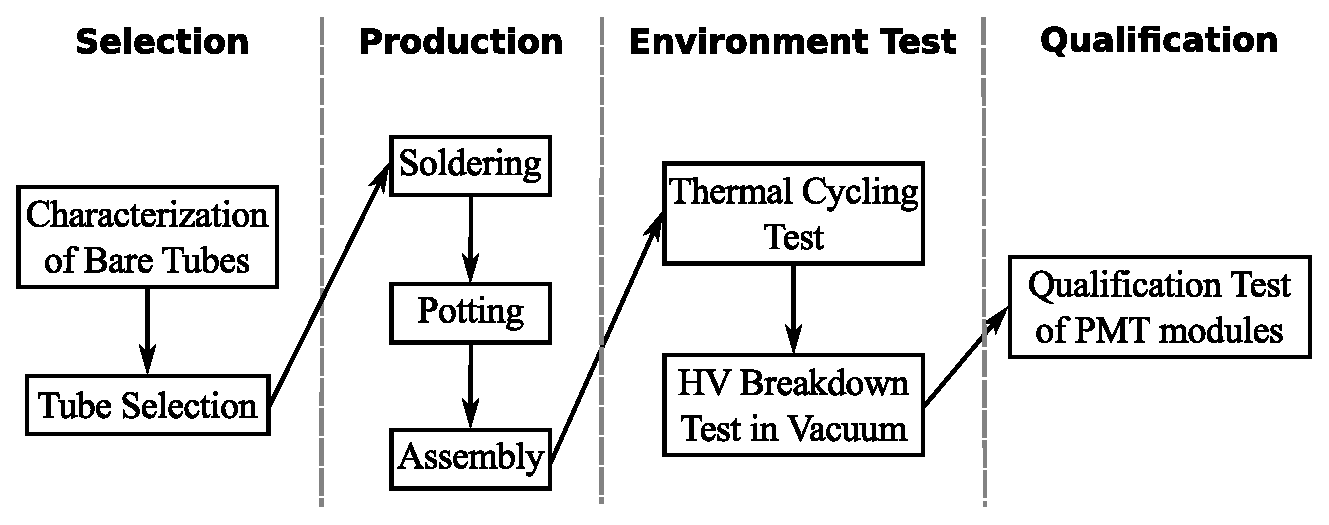
\includegraphics[width=0.95\textwidth]{chap/construction/fig/pmt_production_procedure.eps}
	\caption{PMT组件的生产流程}
	\label{fig:construction:pmt_production_procedure}
\end{figure}

\subsection{结构简介}
\label{sec:construction:pmt_assembly}

\subsection{生产流程}
\label{sec:construction:pmt_procedure}
\begin{enumerate}
	\item PMT的base焊接,信号线+信号头。
	\item 检测:电压、电容。
	\item 灌胶。
	\item 高低温循环。
	\item 真空高压测试。
	\item PMT测试平台测试
\end{enumerate}

\section{塑闪单元条的生产}
\label{sec:construction:bar_production}
测试与筛选过程与PMT正好相反,因为单元条需要包装后才能测试。

\subsection{单元条的包装与测试}
\label{sec:construction:bar_wrapping_and_test}

\subsection{单元条的筛选}
\label{sec:construction:bar_selection}
尺寸复核
热膨胀系数
技术衰减长度:平滑否-包装是否好,两端相差较大也踢出,大于一个值
响应均匀性
探测效率
MPV响应?

\section{探测器整体组装}
\label{sec:construction:psd_assembly}

\subsection{PMT与塑闪单元条的匹配}

\begin{enumerate}
	\item 布单元条。
	\item PMT组件加套筒和播磨合金
	\item 上PMT。
	\item 宇宙线测试。
	\item 上高压扇出板
	\item 上FEE盒子(焊接定位用),上FEE转接板
	\item 上高压接头
	\item 正式上FEE盒子
	\item 上FEE电路板
	\item 上顶板
\end{enumerate}
